\documentclass[a4paper,twoside]{article}
\usepackage[T1]{fontenc}
\usepackage{graphicx}
\usepackage{calc}
\usepackage{amssymb}
\usepackage{amsmath}
\usepackage{pslatex}
\usepackage{apalike}
\usepackage{booktabs}
\usepackage{algorithm2e}
\usepackage[bottom]{footmisc}
\usepackage[hidelinks,breaklinks]{hyperref}
\usepackage{SCITEPRESS}
\hypersetup{pdftitle={Linking Candidate Coverage to Decision Quality: A Framework for LLM Planning Evaluation},pdfauthor={Alexander V. Mantzaris and James H. Korris},pdfsubject={Revised ICAART 2027 position paper},pdfkeywords={LLM Planning, Semantic Validation, Evaluation},pdfcreator={LaTeX}}

\begin{document}
\title{Linking Candidate Coverage to Decision Quality: A Framework for LLM Planning Evaluation}
\author{\authorname{Alexander V. Mantzaris\sup{1} and James H. Korris\sup{2}}
\affiliation{\sup{1}Dr. Yvette Kanouff School of Data, Mathematical, and Statistical Sciences,\\
UCF, 4000 University Blvd, Orlando, FL, USA}
\affiliation{\sup{2}Creative Technologies Inc.}
\email{alexander.mantzaris@ucf.edu, james.korris@cretecinc.com}}
\keywords{LLM Planning, Semantic Validation, Candidate Coverage, Decision Correctness, Evaluation.}
\abstract{A traveler might ask a planning assistant for a journey arriving by a certain time with at most one transfer. A language model translates the request into machine checkable requirements that planning software uses to choose a journey. Confusing the arrival deadline with a departure deadline could produce a journey that passes those checks yet arrives late. An overall success rate cannot explain whether the system understood the request or selected well among possible translations. We propose an evaluation framework examining whether available journeys test the requirements, whether a correct translation was considered, whether example journeys distinguished relevant alternatives, and whether the selected outcome satisfied the request. Two exploratory transit case studies show how these measurements separate limited opportunities to change validation behavior from difficulties using available correct translations. Greater availability of matching translations did not necessarily increase final accuracy. Using constructed requests over published schedules and provisional reference requirements, the analysis connects interpretation, selection, outcomes, and computational cost. These measurements provide a structured basis for diagnosing outcomes and choosing which component to investigate next.}
\onecolumn \maketitle \normalsize \setcounter{footnote}{0} \vfill

\section{\uppercase{Position and Contribution}}
\label{sec:position}
\noindent A traveler asks for a journey arriving by 09:00 with at most one transfer. A language model translates this request into machine checkable constraints, and a planner chooses a journey. Several candidate formalizations may be checked against concrete example journeys. Confusing arrival with departure can admit late journeys, yet the wrong formalization might still select an on-time plan. Conversely, a mistaken judgment of an example can reject a correct formalization. Final accuracy alone does not separate these cases.
We propose three contributions: a framework linking candidate coverage and final correctness on the same requests; two exploratory transit studies showing what these measures explain; and a reproducible procedure for clause tests, validation traces, and cost accounting. Candidate coverage asks whether any generated formalization matches reference requirements over a stated journey pool. Final correctness asks whether the returned outcome satisfies them.

\subsection{Relationship to Prior Evaluation Work}

This is an LLM-as-formalizer setting: a model translates a request and a symbolic planner solves its constraints \cite{tantakoun}. Prior comparisons identify a translation bottleneck \cite{amonkar}; we examine how multiple candidates lead to final decisions.
Semantic Self-Verification checks formalizations using concrete instances \cite{ssv}. Its coverage measures receipt of verification; ours measures whether a reference-matching candidate was generated.
ARTEMIS uses distinguishing traces and human validation \cite{artemis}. Our witness selector, which chooses the next journey to judge, adapts this idea to finite journey pools and model judgments.
Sampling diversity work distinguishes generating a correct solution from selecting it \cite{diversity}. VERGE reports a formalization funnel, failure modes, and token-matched comparisons \cite{verge}. Our contribution connects such measurements to clause tests and joint candidate coverage and final correctness.

\section{\uppercase{A Linked Evaluation Framework}}
\label{sec:framework}

\noindent A \emph{candidate formalization} (or candidate) is a machine checkable translation of a request. We call it \emph{well-formed} when it passes syntax, type, unit, entity, and source-span checks; this does not mean it correctly expresses the request. Algorithm~\ref{alg:pipeline} describes the elimination-only procedure evaluated here. A \emph{witness} is a journey on which surviving candidates disagree. The witness selector chooses which such journey to show the judge; final candidate choice is a separate step.

\begin{algorithm}[ht]
\caption{Candidate generation, validation, and final choice}
\label{alg:pipeline}
\KwIn{Request $x$, ordered journey pool $J_x$, sample allowance $k$, judgment allowance $b$, token allowances (Study~2)}
Generate up to $k$ attempts within the token allowance; retain well-formed candidates and merge candidates with identical pool behavior\;
Save this pre-validation set $\mathcal C_x$; compute each candidate's deterministic plan with Z3\;
Set survivors $A\leftarrow\mathcal C_x$, used journeys $U\leftarrow\emptyset$\;
\For{at most $b$ judgments}{
Find unused separating journeys; stop if none remain or the token allowance prevents a call\;
Choose the highest-scoring journey $w$ (Eq.~\ref{eq:scores}); add $w$ to $U$\;
Ask the model to judge $w$ against $x$\;
If the label is definite, remove candidates disagreeing with it; otherwise retain $A$\;
}
Return the saved plan/status of the first survivor in generation order; if none exist, return an explicit failure status\;
\end{algorithm}

Malformed judgments count as uncertain. Each queried witness remains used, even after uncertainty. Because a separating witness has both accepting and rejecting survivors, either definite label leaves at least one survivor. These studies perform no repair or replacement; a \emph{candidate update} only removes candidates. A \emph{validation sequence} is the ordered list of queried journeys and labels. A \emph{shared state} means the same survivors and used journeys.

Let $x$ be a request and $J_x$ its finite journey \emph{pool} (also called the planning universe). Published schedules and public scenario metadata---endpoints, segment names, service date, and time horizons---define $J_x$ before candidate generation. Each candidate $C$ assigns a Boolean acceptance value to each journey $w$. Its \emph{behavioral signature}, or truth vector, is the list of these values in the fixed pool order:
\begin{equation}
  \sigma_{J_x}(C)=(C(w))_{w\in J_x}.
\end{equation}
Candidates with the same signature form one behavioral class; the earliest generated representative is retained. A candidate set for one request is also called a bundle. Matching signatures establish equivalence only within $J_x$, not source fidelity. Let $R_x$ denote the separately specified reference evaluator; its provisional status matters for all measurements below.

\subsection{Candidate Coverage and Final Correctness}

A \emph{checkpoint} is a sample allowance fixed before evaluation (four attempts in Study 1; two, four, or eight in Study 2). $\mathcal C_x$ contains all well-formed candidates generated up to that checkpoint, after deduplication but \emph{before validation}. It includes candidates later eliminated. Define candidate coverage as
\begin{equation}
 G_x=\mathbf{1}\{\exists C\in\mathcal{C}_x:
                 \sigma_{J_x}(C)=\sigma_{J_x}(R_x)\}.
\end{equation}
Let $S_x=1$ when the final output is a journey satisfying $R_x$, or correctly concludes that no journey in $J_x$ satisfies it. Timeouts, malformed outputs, abstentions, and false infeasibility claims have $S_x=0$ and are reported separately.

The joint cells distinguish a match followed by success, $(1,1)$; failure despite a match, $(1,0)$; success without a match, $(0,1)$; and failure without a match, $(0,0)$. Coverage and correctness totals alone do not determine these cells. A candidate can accept invalid journeys yet select a valid one. For $(1,0)$ cases, inspect judgments, final tie-breaking, and budget limits before assigning a cause. For $(0,0)$ cases, check whether any candidate's selected plan was correct before blaming missing alternatives.

\subsection{Choosing Distinguishing Journeys}

A set is \emph{distinguishable} if some candidates disagree on a pool journey. Let $\pi_i$ be candidate $C_i$'s deterministic plan. Define the cross-rejection count
\begin{equation}
 I_{ij}=\mathbf{1}\{\neg C_j(\pi_i)\}
       +\mathbf{1}\{\neg C_i(\pi_j)\},
\end{equation}
with each missing-plan term set to zero. This count is 0, 1, or 2. A set has a \emph{consequential disagreement} if any pair has $I_{ij}>0$: at least one candidate rejects the other's selected plan. This measures incompatibility, not correctness.

For survivors $A$, let $P_A(w)=\{(i,j):i<j,\ C_i,C_j\in A,\ C_i(w)\ne C_j(w)\}$. A witness partitions $A$ into accepting and rejecting candidates. With positive witness cost $c(w)$, the scores are
\begin{equation}
\begin{split}
 q_{\rm bal}(w)&=|P_A(w)|/c(w),\\
 q_{\rm con}(w)&=\sum_{(i,j)\in P_A(w)}(1+I_{ij})/c(w).
\end{split}
\label{eq:scores}
\end{equation}
Choose the unused $w\in J_x$ with nonempty $P_A(w)$ and largest score; ties use lexicographic journey ID. Both studies set $c(w)=1$ model judgment, so division does not affect ranking. Token accounting is separate. Weighting aims to spend judgments on disagreements that could change the selected plan's acceptability. It need not improve correctness.
If all pair weights are equal, the scores differ by a positive constant factor and rank witnesses identically. This always holds for two candidates. Identical validation sequences also require the same judgments and updates at shared states.

\subsection{Testing Requirements in the Pool}

A requirement appearing in a request does not establish that the pool tests it. A reference clause \emph{varies} if it accepts some journeys and rejects others; otherwise it is constant. A varying clause is \emph{masked} if it excludes no journey satisfying all other clauses. These are different ways a pool can fail to expose a distinction. More generally, an uninformative pool can make different formalizations behave alike.
Stronger contrasts may be necessary. Testing ordered visits requires different orders with the same stops. Variation due only to stop presence does not test order. Check these contrasts separately for each requirement family, such as time, transfers, modes, or visits. We call this \emph{clause testing}, reserving \emph{candidate coverage} for $G$.


\section{\uppercase{Two Exploratory Transit Studies}}
\label{sec:setup}

\noindent Both studies use constructed requests over a frozen September 2026 TriMet GTFS feed \cite{trimet,gtfs}, not passenger records or observed movements. Service is evaluated on 14 September 2026 in \texttt{America/Los\_Angeles}, with calendars, exceptions, service-day seconds, and inclusive boundaries.
A pre-output route-selection rule selected connected bus routes 2, 4, and 17 in downtown Portland. Journeys have at most two rides per segment and exact-stop transfers with a 120-second minimum. Walking, through-service, capacity, and accessibility guarantees are excluded. Public endpoints and horizons define the universe; references and predictions never prune it. Plans optimize arrival, boardings, departure, then journey ID. Enumeration caps make every feasibility and equivalence claim pool-relative.
The typed language has grammar $E::=\mathrm{atom}(o,s,v,u)\mid\mathrm{all}(E_1,\ldots,E_n)\mid\mathrm{not}(E)$. An atom has an operator, segment scope, value, and unit. Time bounds use nonnegative integer seconds; transfers use counts; mode and visit operators use nonempty lists of modes and stop IDs. For example, the complete formula
\begin{quote}\small
\texttt{\{"kind":"atom","op":"arrive\_by",}\newline
\texttt{"scope":"outbound","value":32400,}\newline
\texttt{"unit":"seconds"\}}
\end{quote}
means outbound arrival by 09:00, inclusive. Conjunction combines requirements; negation reverses acceptance. Separate reference code evaluates outcomes. The companion reproducibility document gives the full JSON schema, response wrapper, prompts, and examples.


\subsection{Shared Model and Validation}

Both use Qwen2.5-7B-Instruct \cite{qwen}, revision \texttt{a09a35458c702b33eeac\allowbreak{}c393d103063234e8bc28}, BF16, Transformers 4.51.3, and PyTorch 2.8.0/CUDA 12.8. Sampling uses temperature 0.7, top-$p$ 0.95, top-$k$ 20, repetition penalty 1.05, and at most 768 output tokens. Each base has one replicate.
The judge receives only the request and a deterministic journey description with times, stops, and transfers. It returns satisfied, violated, or uncertain; definitive labels eliminate inconsistent candidates. Translation and judgment use the same model in fresh invocations, not an independent truth oracle. Comparisons use elimination without repair-generated candidates.
Requests and reference rules were constructed together by assistant-authored template code before generation, using selected scheduled journeys to set bounds. A separate narrow grammar re-parsed the request wording without importing the constructor or candidate compiler; an independent evaluator checked reference outcomes. Study 1's automated audit checked all 48 requests, times, scopes, entities, and pool journeys, then rescored 432 saved outputs without changing any category. These checks found no clear reference error, but neither the references nor disagreeing judgments received independent human adjudication. All error attributions below are relative to these provisional references.
The preserved outputs come from this project's September 2026 Qwen runs: \texttt{stage2-pilot-v1} and \texttt{stage3-fresh}. This paper reanalyses those runs; revisions used no new experimental inference.

\subsection{Study 1: Selecting Validation Examples}

The selector study comprises 48 fresh base requests, one replicate each, using 07:00 to 10:00 schedules. Eight requests each target timing, transfers, mode exclusions, outbound/return scope, ordered visits, and infeasibility. Forty are reference-feasible and eight infeasible within their pools. The 48 pools contain 4,366 journey memberships, capped at 64 per single segment and 256 for combined journeys; 40 pools were truncated.
Each request supplies the same four raw candidate attempts to the balanced and consequence-weighted selectors. The witness cost is one. Budgets of zero, one, two, and four judgments reuse the initial part (prefix) of each validation sequence. Fixed before the fresh run on 12 September 2026, the throughput rule used the first 16 translations' latency to reduce two replicates to one. For $n$ requests and $r$ replicates, it forecast $N=n(13r+3)$ calls and $Nt+2nr+120$ seconds, with $t=1.5\max(p_{95},2.8164)$ seconds. It required remaining time to cover this forecast and $N\leq1500-64$; otherwise it reduced replicates first, then removed six-request blocks. All 48 requests fit with one replicate. No candidate errors were deliberately injected into the experiment.

\subsection{Study 2: Sampling Interpretations}

The sampling study uses 32 new base requests and 10:00 to 13:00 schedules. Prior origin destination groups and their reverses are excluded, but routes, stops, date, and templates overlap. This separate protocol is not an independent replication. Twenty-eight requests are feasible and four infeasible. Timing, transfer, and scope requirements were selected for informative contrasts; modes and ordered visits were omitted. All 56 reference clauses vary and have conditional exclusions. Pools retain at most 128 journeys per segment and 256 combined journeys.
Independent sampling repeats the base prompt. Diversified sampling adds fixed checks of timing, scope, negation, transfers, omissions, and literal reading. Solver-guided sampling adds summaries of prior formulas and their full and clause signatures, plus a concrete journey when space permits. Repeated readings are permitted. Feedback excludes references and judgments and is capped at 6,000 characters. Exact prompts and feedback formatting appear in the companion and source files (Section~\ref{sec:availability}). All arms share source-only time normalization: an existing temporal atom's value becomes $3600h+60m+s$ only when exactly one source time matches its operator and scope. Missing constraints, wrong operators, and wrong scopes are unchanged.
The first two samples are shared across arms. Each complete sampling sequence is generated before evaluating its first 2, 4, and 8 attempts, each with balanced witness selection and at most two judgments. Identical allocations permit 35,000 generation tokens per request and 4,000 validation tokens per prefix, counting input plus output. Calls require enough allowance for their input and maximum output. No allowance was exhausted; eight attempts stopped every sampling sequence. These are equal ceilings, not equal actual compute.



\section{\uppercase{Explanatory Value in Two Studies}}
\label{sec:findings}

\noindent Base requests are the observational unit; study denominators remain separate. Attempts, checkpoints, and reused judgments are not independent observations. Joint outcomes and privileged label replay derive from preserved outputs.

\subsection{Characterizing Selection Opportunity}

In Study 1, 25 of 48 candidate sets contain distinguishable candidates, and 18 contain consequential disagreements. Figure~\ref{fig:opportunity} connects these nested sets to observed validation behavior. Fourteen consequential candidate sets have uniform pair weights. Of the remaining four, two select the same initial witness through shared tie breaking and then have at most two surviving classes. Two validation sequences differ, with equal correctness and one different final plan identifier. 

\begin{figure*}[t]
\centering
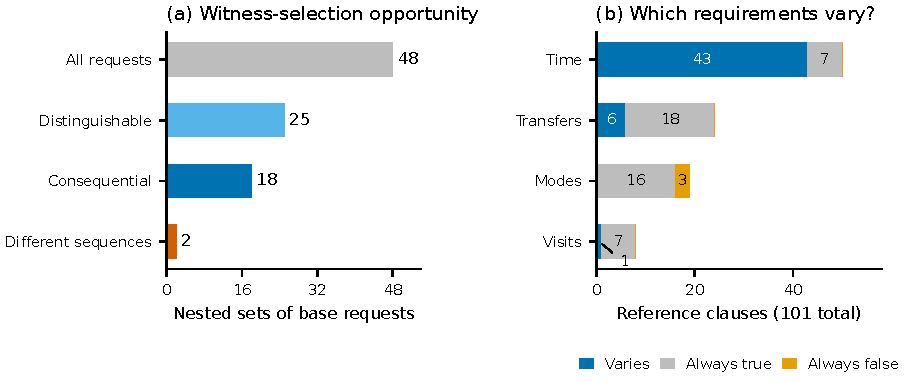
\includegraphics[width=\textwidth]{figures/selector-opportunity.pdf}
\caption{Study 1: witness-selection opportunity and clause tests. Only two of 48 requests yield different validation sequences. Uniform pair weights and shared tie-breaking explain most identical choices. Of 101 reference clauses, 51 are constant; visits never test order independently of stop presence.}
\label{fig:opportunity}
\end{figure*}

Both selectors resolve 31/48 requests at budget zero and 33/48 at budgets 1, 2, and 4: three recoveries and one deterioration, a net 4.17-point gain. This is a validation gain, with no weighting advantage. In the deteriorated case, a correct negative judgment removes a wrong formalization whose initial plan was valid, exposing a dependency between candidate coverage and preservation of a successful decision.
Each selector returns 30/40 valid feasible plans, five invalid plans, and five false infeasibility conclusions. It identifies 3/8 infeasible requests; five give invalid interpretation outputs. No unresolved or infrastructure failures occur. Budget two adds four judgments per method but changes no plan; budget four adds no judgments. No further separating witnesses remain. Oracle-witness replay reaches 35/48 for both selectors, identifying a shared opportunity in validation rather than an advantage of weighting.
Clause checks identify which requirements the benchmark exercises. Of 101 reference clauses, 50 vary, 48 are always satisfied, and three always violated. Six of 24 transfer clauses vary although 45/48 pools offer zero and one transfer journeys; the two-ride bound makes an at-most-one-transfer clause vacuous. All 19 mode clauses are constant, and visits never distinguish ordering beyond stop presence. Removing enumeration caps increases memberships to 77,871 without adding candidate classes or witness partitions for the saved bundles. 



\subsection{Candidate Coverage and Final Decisions}

In Study 2, diversified sampling reaches 31/32 candidate coverage compared with 27/32 for independent sampling, while both produce 28/32 correct final outcomes. Figure~\ref{fig:cost} separates candidate coverage and final correctness against consumed tokens. All arms begin at 25/32 candidate coverage and correctness. Solver-guided sampling stays there through eight attempts, adding no matching behavior after the shared samples. Mean distinct signatures are 1.41, 1.59, and 1.19 for independent, diversified, and solver-guided sampling. 

\begin{figure*}[t]
\centering
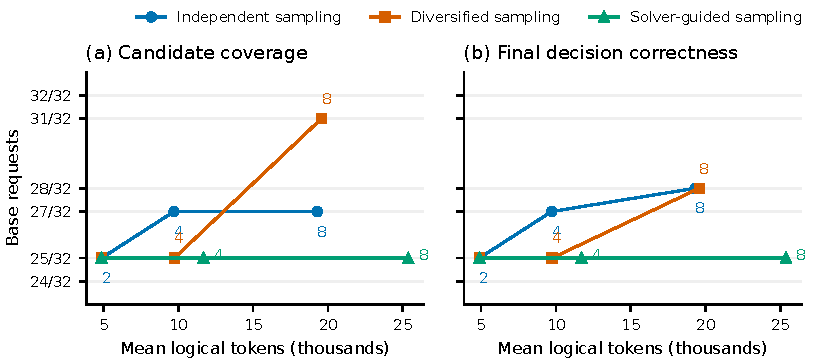
\includegraphics[width=\textwidth]{figures/cost-outcomes.pdf}
\caption{Study 2: candidate coverage and final correctness versus mean logical input plus output tokens. Labels mark 2, 4, and 8 attempts; lines connect observed checkpoints. Generation and checkpoint validation are charged. The first two samples are shared; no token allowance is exhausted.}
\label{fig:cost}
\end{figure*}

Request-level pairing reveals a distinction behind equal totals: independent sampling wins on one request, loses on one, and ties on 30 against diversified sampling. Solver guided sampling has zero wins, three losses, and 29 ties against each baseline, with different losing sets. Its correctness difference is $-9.38$ percentage points in each comparison. A 10,000 draw base-request bootstrap gives a descriptive 95\% interval of $[-21.88,0]$ points; independent minus diversified gives $[-9.38,9.38]$. 
The baselines return 24/28 valid feasible plans; solver-guided sampling returns 21/28. All identify four infeasible requests correctly; remaining outputs are invalid plans. No final output is unresolved, malformed, or an infrastructure failure; two malformed candidate attempts remain charged. Before fresh outputs on 13 September 2026, the protocol fixed continuation thresholds of at least ten percentage points more candidate coverage and five points more final correctness than each baseline. Solver-guided sampling met neither threshold.



\subsection{Locating Candidate-to-Decision Transitions}

\begin{figure}[t]
\centering
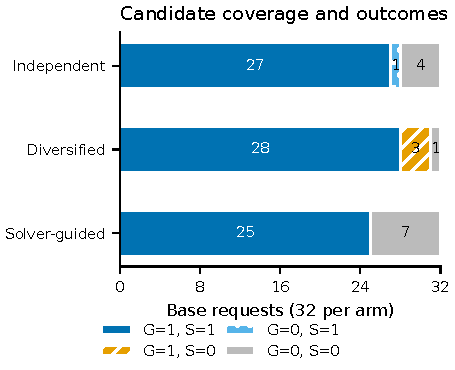
\includegraphics[width=\columnwidth]{figures/joint-outcomes.pdf}
\caption{Joint candidate coverage $G$ and final correctness $S$ at eight attempts (32 requests per arm). Off-diagonal cells show three diversified-sampling losses despite a match and one independent-sampling success without a match. All counts use provisional references.}
\label{fig:joint}
\end{figure}

Figure~\ref{fig:joint} shows how candidate coverage relates to final outcomes. In $(1,1),(1,0),(0,1),(0,0)$ order the final counts are $(27,0,1,4)$ for independent, $(28,3,0,1)$ for diversified, and $(25,0,0,7)$ for solver-guided sampling. At four attempts, diversification has $(24,1,1,6)$ as equal marginal coverage and correctness of 25 conceal both off-diagonal outcomes. 
Relative to the provisional references, trace inspection identifies disagreeing judgments eliminating the match in all three diversified final $(1,0)$ cases, 2 false positives and one false negative. A fourth loss appears at four attempts. Each final case ends with one class, so an unresolved tie or unused validation opportunity is not the immediate cause. Reference labels recover all three under the same evaluation. Across selected witnesses, 11/19 distinct Study 2 judgments and 7/31 Study 1 judgments disagree with provisional references. These cases were not independently adjudicated and are not general judge accuracy estimates. 

\begin{figure*}[t]
\centering
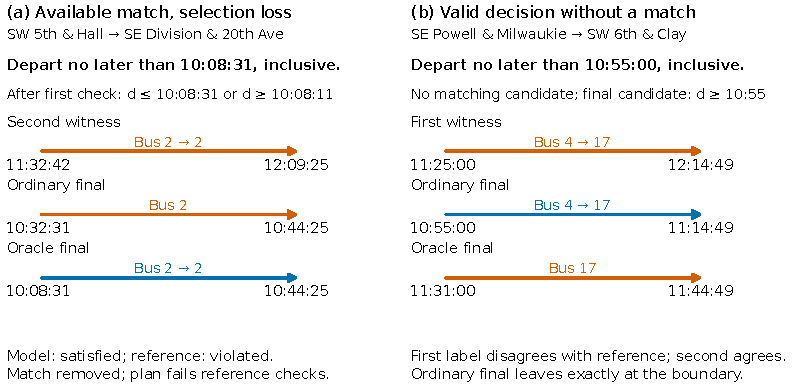
\includegraphics[width=\textwidth]{figures/worked-transit.pdf}
\caption{Study 2 examples: losing a matching candidate (left) and succeeding without one (right). ``Oracle'' uses reference labels. Correctness is relative to provisional references. Times are local scheduled times on 14 September 2026; arrows show endpoints, not a scaled time axis.}
\label{fig:worked}
\end{figure*}

The left example requests departure by 10:08:31. A correct first judgment leaves the matching upper bound and a wrong lower bound. Accepting a second witness departing at 11:32:42 removes the match and yields a 10:32:31 plan. Reference-label replay returns a valid 10:08:31 departure. 

\subsection{Distinguishing Oracle Measurements}

Oracle witness replay substitutes reference labels while retaining bounded elimination and the first surviving candidate. Correctness is 27/32, 31/32, and 25/32: equal to coverage totals here, but measuring a different procedure.
Figure~\ref{fig:worked} (right) explains independent sampling's 28 ordinary versus 27 oracle witness successes. The request requires departure by 10:55; no candidate matches throughout the pool. A wrong positive on an 11:25 departure removes one candidate. A correct second positive retains a lower-bound candidate, whose optimal plan leaves exactly at 10:55 and satisfies the request. Reference-label first witness rejection instead retains a candidate producing an 11:31 departure. Thus reference labels can change the elimination path and lose a valid decision: this procedure is not an accuracy ceiling.
A separate diagnostic asks whether \emph{any existing candidate's selected output} is correct: 28/32, 31/32, and 25/32 at eight attempts. This best-of-candidate-outputs measure is restricted to existing plans; it differs from both $G$ and reference-label replay.

\subsection{Relating Inference Cost to Discovery}

Final prefix logical input/output tokens total 617,643, 626,497, and 811,760 for independent, diversified, and solver-guided sampling across 32 requests each. Solver guided overhead is 31.43\% and 29.57\%, relative to the corresponding baseline's consumed generation plus validation total. Logical calls are 266, 269, and 262. The extra tokens produced no additional matching candidates.
Across checkpoints, generation is counted once per sampling sequence and judgments once per checkpoint: 833 logical calls and 2,081,931 tokens. Caching reduces actual fresh compute to 659 calls and 1,743,059 tokens. The companion records GPU times and development costs. Shared outputs retain full per-arm logical charges.



\section{\uppercase{Applying the Framework}}
\label{sec:recommendations}

\noindent For each request, retain its pool, reference rules, generated candidates, signatures, selected plans, witnesses, judgments, and costs. Report joint $(G,S)$ cells and output categories, then inspect the traces behind them.
First, test clauses before evaluating models: include journeys on both sides of a time or transfer limit, and different visit orders with the same stops. Larger pools alone do not ensure useful contrasts.
Second, use the joint cells to choose what to inspect. Diversification increased candidate coverage without increasing final correctness. The three traced losses point to validation as a component to investigate, conditional on the references. Independent review of those references and disputed judgments should precede a claim about judge error. A $(0,1)$ outcome preserves a correct plan's value without certifying its formalization.
Third, report tokens, logical calls, caching, and stopping reasons alongside sample allowances. Here they reveal feedback costs without additional matches and extra judgments without changed plans.
The framework supplies diagnostic information; it has not itself been shown to improve accuracy or reduce cost. The results do not support expanding the tested weighting or feedback variants.


\section{\uppercase{Limitations}}
\label{sec:limitations}


\noindent The studies contain 48 and 32 requests, one model, and one replicate. Constructed wording, overlapping services, and a shared translation/judgment model limit generalization. Different protocols prevent pooling the studies. Bootstrap intervals exclude annotation uncertainty, route dependence, and variation over models and prompts.
References remain provisional: the 80-request worksheet has no completed human-review decisions. Systematic wording errors could affect $G$ and $S$ together, so disputed judgments require independent review.
All claims concern bounded pools, not the full network. Non-bus services, midnight, and daylight saving are untested. Transfer clauses can be vacuous and visits do not independently test order. Study 2 improves clause tests without resolving these limits. Matching signatures can hide differences for which the pool lacks examples; clause associations with source wording may also be unavailable.
Stronger judges, other prompts, and broader pools could change the comparisons. Repeated lower-bound readings do not establish feedback anchoring. This framework developed from exploratory studies, not a preregistered reporting hypothesis; its value across models and domains remains untested.


\section{\uppercase{Conclusion}}
\label{sec:conclusion}

\noindent Reporting candidate coverage and final correctness jointly explains differences hidden by aggregate accuracy. Clause tests show what the benchmark exercises, while validation traces and costs show how available candidates are used. In these studies, weighting rarely changed witness choices, and greater candidate coverage did not guarantee better final decisions. Next, disputed reference cases need independent review, followed by tests with other models and more varied pools. These steps would test whether the same diagnosis remains useful beyond this setting.


\subsection*{Code and Data Availability}
\label{sec:availability}
Code, prompts, constructed requests, provisional references, frozen protocols, and compact results are available in the \href{https://github.com/mantzaris/LLMplanningContraintsDecision}{project repository}. The companion \texttt{reproducibility.pdf} documents exact templates and commands. The frozen feed and full raw generation logs remain in project storage, outside the public repository; full historical replay requires those files. Compact tables and figures can be inspected without them.

\subsection*{AI Assistance Disclosure}
\label{sec:ai}
OpenAI Codex \cite{codex} assisted with the code and environment setup.


\begin{thebibliography}{99}
\bibitem[Amonkar et~al., 2026]{amonkar}
Amonkar, R., Kayan, C.~E., Lai, Q., Le~Bras, R., and Zhang, L. (2026).
A reality check of language models as formalizers on constraint satisfaction problems.
\emph{arXiv:2505.13252v6}. Preprint; first submitted 2025.
\href{https://arxiv.org/abs/2505.13252v6}{doi:10.48550/arXiv.2505.13252}.

\bibitem[GTFS, 2026]{gtfs}
GTFS (2026). Schedule reference.
\url{https://gtfs.org/documentation/schedule/reference/}. Accessed 13 September 2026.

\bibitem[Mendoza et~al., 2026]{artemis}
Mendoza, D., Mavridou, A., Katis, A., and Trippel, C. (2026).
Automating requirements formalization: Using LLMs and low-complexity distinguishing traces for semantic validation.
In \emph{48th IEEE/ACM International Conference on Software Engineering (ICSE)}.
\href{https://doi.org/10.1145/3744916.3787815}{doi:10.1145/3744916.3787815}.

\bibitem[OpenAI, 2026]{codex}
OpenAI (2026). Codex. AI assistance tool.
\url{https://openai.com/codex/}. Accessed 13 September 2026.

\bibitem[Qwen Team, 2024]{qwen}
Qwen Team (2024). Qwen2.5-7B-Instruct: Official model card.
\url{https://huggingface.co/Qwen/Qwen2.5-7B-Instruct}. Accessed 13 September 2026.

\bibitem[Raza and Milic-Frayling, 2025]{ssv}
Raza, M. and Milic-Frayling, N. (2025).
Instantiation-based formalization of logical reasoning tasks using language models and logical solvers.
In \emph{Proceedings of IJCAI-25}, pages 4633--4641.
\href{https://doi.org/10.24963/ijcai.2025/516}{doi:10.24963/ijcai.2025/516}.

\bibitem[Singh et~al., 2026]{verge}
Singh, V., Cassel, D., Weir, N., Feng, N., and Bayless, S. (2026).
VERGE: Formal refinement and guidance engine for verifiable LLM reasoning.
\emph{arXiv:2601.20055v2}. Preprint.
\href{https://arxiv.org/abs/2601.20055v2}{doi:10.48550/arXiv.2601.20055}.

\bibitem[Tantakoun et~al., 2025]{tantakoun}
Tantakoun, M., Muise, C., and Zhu, X. (2025).
LLMs as planning formalizers: A survey for leveraging large language models to construct automated planning models.
In \emph{Findings of the Association for Computational Linguistics: ACL 2025}, pages 25167--25188.
\href{https://doi.org/10.18653/v1/2025.findings-acl.1291}{doi:10.18653/v1/2025.findings-acl.1291}.

\bibitem[TriMet, 2026]{trimet}
TriMet (2026). GTFS schedule data.
\url{https://developer.trimet.org/GTFS.shtml}. Feed version 20260823-20260910-0900; acquired September 2026.

\bibitem[Wang et~al., 2026]{diversity}
Wang, T., Liu, Z., Chen, Y., Light, J., Liu, W., Chen, H., Zhang, X., and Cheng, W. (2026).
On the effect of sampling diversity in scaling LLM inference.
\emph{arXiv:2502.11027v5}. Preprint; first submitted 2025.
\href{https://arxiv.org/abs/2502.11027v5}{doi:10.48550/arXiv.2502.11027}.
\end{thebibliography}
\end{document}
